\documentclass[tikz,border=14pt]{standalone}
\usepackage[T1]{fontenc}
\usepackage{tgheros}
\usepackage{sfmath}
\usepackage{amsmath}
% % \usepackage{fontawesome5} (Removed for publication-grade academic typography) (Removed for publication-grade academic typography)
\usepackage{tikz}
\usetikzlibrary{arrows.meta,positioning,shapes.geometric,fit,backgrounds,calc}
\usepackage{xcolor}

\renewcommand{\familydefault}{\sfdefault}

% Harvard Crimson & ETH Zurich Academic Semantic Palette
\definecolor{harvardcrimson}{HTML}{A51C30}
\definecolor{ethdarkblue}{HTML}{1F407A}
\definecolor{ethblue}{HTML}{215CAF}
\definecolor{ethpetrol}{HTML}{007A87}
\definecolor{ethbronze}{HTML}{B87333}
\definecolor{ethpurple}{HTML}{5B4B8A}
\definecolor{ethslate}{HTML}{475569}
\definecolor{cardbg}{HTML}{F8FAFC}
\definecolor{cardborder}{HTML}{CBD5E1}

\newcommand{\mputag}[1]{\colorbox{ethbronze!15}{\scriptsize\bfseries\color{ethbronze}\,#1\,}}
\newcommand{\mcutag}[1]{\colorbox{ethpetrol!15}{\scriptsize\bfseries\color{ethpetrol}\,#1\,}}

\begin{document}
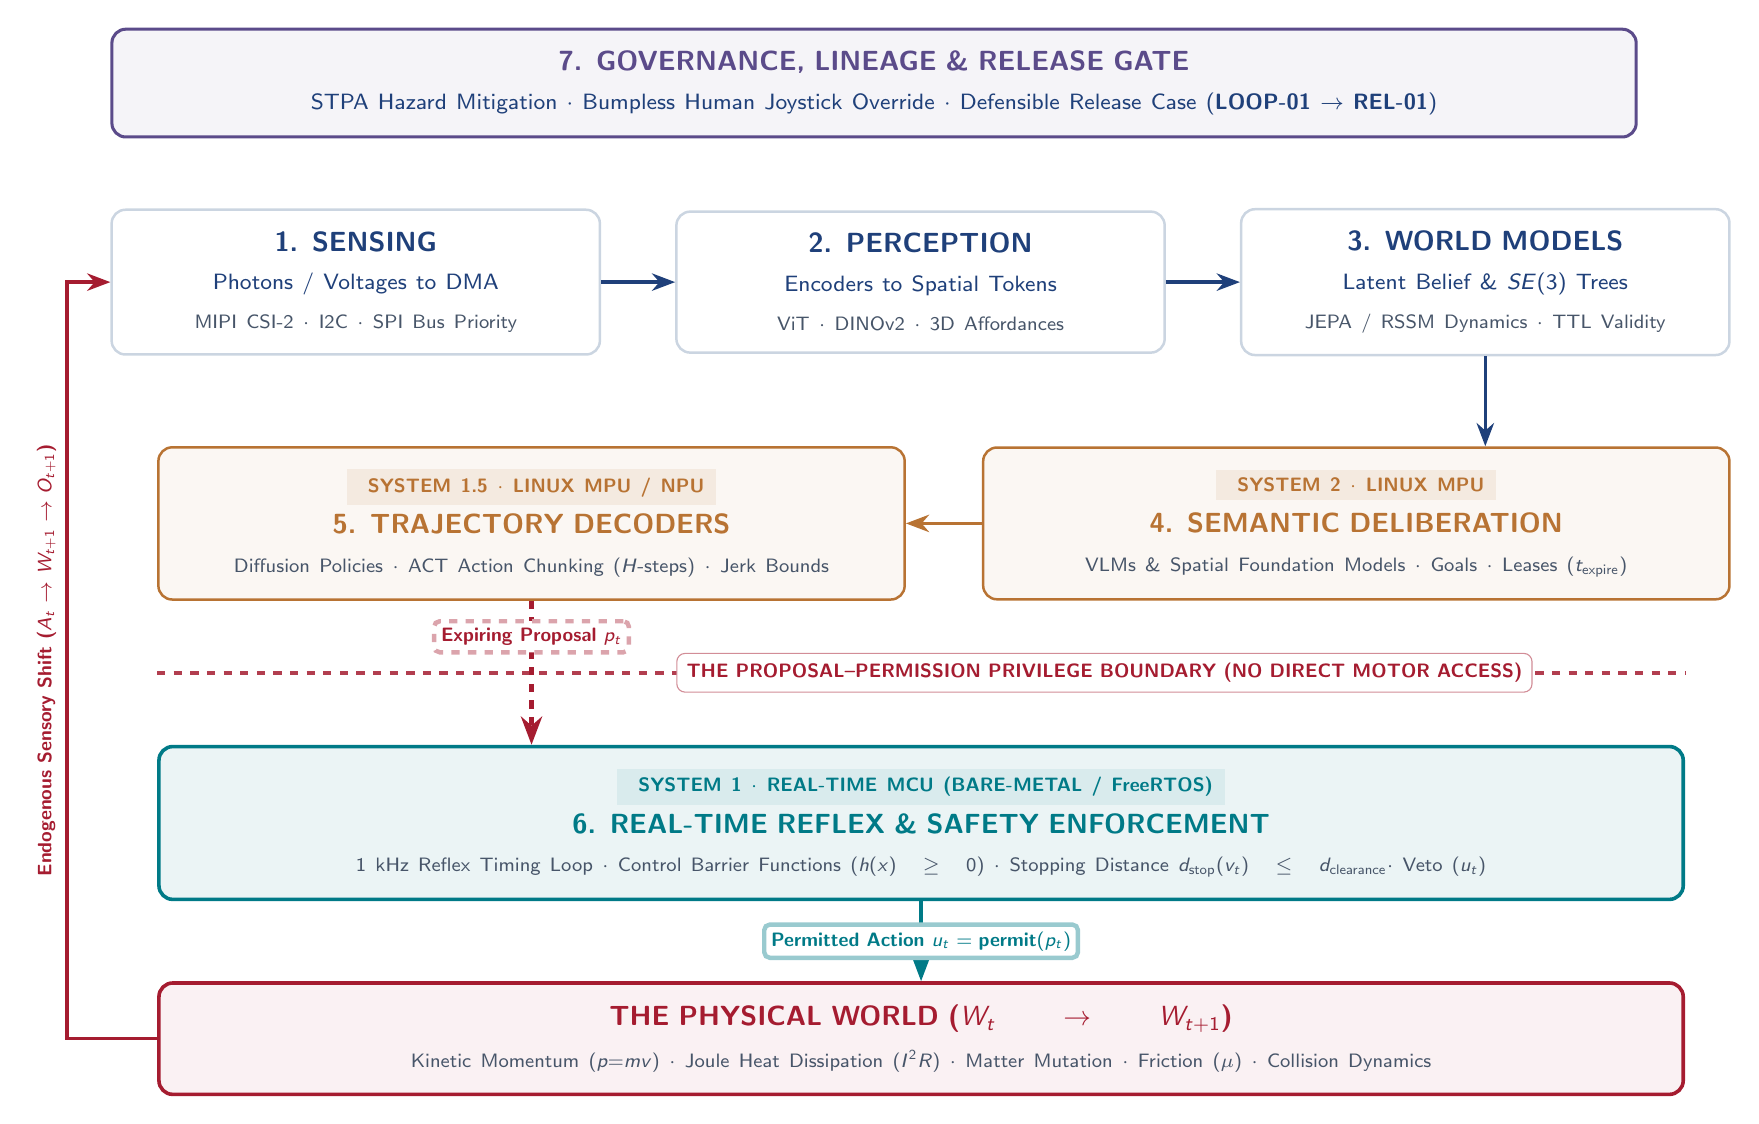
\begin{tikzpicture}[
  font=\sffamily,
  >=Stealth,
  organ/.style={
    draw=cardborder,
    fill=white,
    rounded corners=5pt,
    line width=0.9pt,
    inner sep=8pt,
    align=center,
    text=ethdarkblue
  }
]

  % Top Banner: Stage 7 Governance
  \node[organ, draw=ethpurple, fill=ethpurple!6, text width=7.4in, line width=1.1pt] (s7) {
    {\normalsize\bfseries\color{ethpurple} 7. GOVERNANCE, LINEAGE \& RELEASE GATE}\\[2pt]
    {\footnotesize STPA Hazard Mitigation $\cdot$ Bumpless Human Joystick Override $\cdot$ Defensible Release Case (\textbf{LOOP-01} $\to$ \textbf{REL-01})}
  };

  % --- TOP PIPELINE ROW: Ingestion to State ---
  \node[organ, text width=2.22in, below=0.35in of s7.south west, anchor=north west] (s1) {
    {\bfseries\color{ethdarkblue} 1. SENSING}\\[2pt]
    {\footnotesize Photons / Voltages to DMA}\\[2pt]
    {\scriptsize\color{ethslate}MIPI CSI-2 $\cdot$ I2C $\cdot$ SPI Bus Priority}
  };

  \node[organ, text width=2.22in, right=0.37in of s1] (s2) {
    {\bfseries\color{ethdarkblue} 2. PERCEPTION}\\[2pt]
    {\footnotesize Encoders to Spatial Tokens}\\[2pt]
    {\scriptsize\color{ethslate}\mbox{ViT} $\cdot$ \mbox{DINOv2} $\cdot$ 3D Affordances}
  };

  \node[organ, text width=2.22in, right=0.37in of s2] (s3) {
    {\bfseries\color{ethdarkblue} 3. WORLD MODELS}\\[2pt]
    {\footnotesize Latent Belief \& $SE(3)$ Trees}\\[2pt]
    {\scriptsize\color{ethslate}JEPA / RSSM Dynamics $\cdot$ TTL Validity}
  };

  % --- MIDDLE PIPELINE ROW: Untrusted Proposal Engine (MPU) ---
  \node[organ, draw=ethbronze, fill=ethbronze!6, text width=3.51in, below=0.45in of s3.south east, anchor=north east] (s4) {
    \mputag{ SYSTEM 2 $\cdot$ LINUX MPU}\\[3pt]
    {\bfseries\color{ethbronze} 4. SEMANTIC DELIBERATION}\\[2pt]
    {\scriptsize\color{ethslate}VLMs \& Spatial Foundation Models $\cdot$ Goals $\cdot$ Leases ($t_{\text{expire}}$)}
  };

  \node[organ, draw=ethbronze, fill=ethbronze!6, text width=3.51in, left=0.38in of s4] (s5) {
    \mputag{ SYSTEM 1.5 $\cdot$ LINUX MPU / NPU}\\[3pt]
    {\bfseries\color{ethbronze} 5. TRAJECTORY DECODERS}\\[2pt]
    {\scriptsize\color{ethslate}Diffusion Policies $\cdot$ \mbox{ACT Action Chunking} ($H$-steps) $\cdot$ Jerk Bounds}
  };

  % --- LOWER ROW: Trusted Real-Time Enforcer (MCU) ---
  \node[organ, draw=ethpetrol, fill=ethpetrol!8, line width=1.3pt, text width=7.4in, below=0.72in of s5.south west, anchor=north west] (s6) {
    \mcutag{ SYSTEM 1 $\cdot$ REAL-TIME MCU (BARE-METAL / FreeRTOS)}\\[3pt]
    {\bfseries\color{ethpetrol} 6. REAL-TIME REFLEX \& SAFETY ENFORCEMENT}\\[2pt]
    {\scriptsize\color{ethslate}1 kHz Reflex Timing Loop $\cdot$ Control Barrier Functions ($h(x) \ge 0$) $\cdot$ Stopping Distance $d_{\text{stop}}(v_t) \le d_{\text{clearance}} \cdot$ Veto ($u_t$)}
  };

  % --- PHYSICAL WORLD ROW ---
  \node[organ, draw=harvardcrimson, fill=harvardcrimson!6, line width=1.3pt, text width=7.4in, below=0.40in of s6.south west, anchor=north west] (world) {
    {\bfseries\color{harvardcrimson} THE PHYSICAL WORLD ($W_t \to W_{t+1}$)}\\[3pt]
    {\scriptsize\color{ethslate}Kinetic Momentum ($p{=}mv$) $\cdot$ Joule Heat Dissipation ($I^2R$) $\cdot$ Matter Mutation $\cdot$ Friction ($\mu$) $\cdot$ Collision Dynamics}
  };

  % Proposal-Permission Privilege Boundary (Red Dashed Line)
  \coordinate (bleft) at ($(s6.north west) + (0, 0.36in)$);
  \coordinate (bright) at ($(s6.north east) + (0, 0.36in)$);
  \draw[dashed, line width=1.3pt, harvardcrimson!85] (bleft) -- (bright);

  % Position badge clearly on the right half so it never collides with the left vertical arrow
  \node[font=\sffamily\bfseries\scriptsize, fill=white, draw=harvardcrimson!50, rounded corners=3pt, inner sep=3.5pt, text=harvardcrimson] 
    at ($(bleft)!0.62!(bright)$) 
    { THE PROPOSAL--PERMISSION PRIVILEGE BOUNDARY (NO DIRECT MOTOR ACCESS)};

  % Clean Un-occluded Feed-forward Data Flow Arrows
  \draw[->, line width=1.2pt, ethdarkblue] (s1.east) -- (s2.west);
  \draw[->, line width=1.2pt, ethdarkblue] (s2.east) -- (s3.west);
  \draw[->, line width=1.2pt, ethdarkblue] (s3.south) -- (s3.south |- s4.north);
  \draw[->, line width=1.2pt, ethbronze] (s4.west) -- (s5.east);
  
  % Vertical Dataflow with White Badge Pills (Positioned safely above dashed line)
  \draw[->, line width=1.6pt, dashed, harvardcrimson] (s5.south) -- node[pos=0.25, fill=white, draw=harvardcrimson!40, rounded corners=2pt, inner sep=2.5pt, font=\sffamily\bfseries\scriptsize\color{harvardcrimson}]{ Expiring Proposal $p_t$} (s5.south |- s6.north);
  \draw[->, line width=1.6pt, ethpetrol] (s6.south) -- node[pos=0.5, fill=white, draw=ethpetrol!40, rounded corners=2pt, inner sep=2.5pt, font=\sffamily\bfseries\scriptsize\color{ethpetrol}]{ Permitted Action $u_t = \text{permit}(p_t)$} (world.north);

  % Closed-loop Endogenous Feedback Arrow
  \draw[->, line width=1.2pt, harvardcrimson] (world.west) -- ++(-0.45in,0) |- (s1.west)
    node[pos=0.25, above, rotate=90, font=\sffamily\bfseries\scriptsize\color{harvardcrimson}, align=center]{ Endogenous Sensory Shift ($A_t \to W_{t+1} \to O_{t+1}$)};

\end{tikzpicture}
\end{document}
